\documentclass[a4paper, amsfonts, amssymb, amsmath, reprint, showkeys, nofootinbib, twoside]{revtex4-1}
\usepackage[english]{babel}
\usepackage[utf8]{inputenc}
\usepackage[colorinlistoftodos, color=green!40, prependcaption]{todonotes}
\usepackage[pdftex, pdftitle={Article}, pdfauthor={Author}]{hyperref}
\usepackage{amsthm}
\usepackage{mathtools}
\usepackage{physics}
\usepackage{xcolor}
\usepackage{caption}
\usepackage{hyperref}
\usepackage{multirow}
\usepackage{amsmath}
\usepackage{amssymb}
\usepackage{graphicx}
\graphicspath{Images}
\usepackage[left=23mm,right=13mm,top=35mm,columnsep=15pt]{geometry} 
\usepackage{adjustbox}
\usepackage{placeins}
\usepackage[T1]{fontenc}
\usepackage{float}
%\usepackage{longtable}
\usepackage{csquotes}
\usepackage{refstyle}
\usepackage{lipsum}
\usepackage{booktabs}

\begin{document}

\title{Study of Compton Scattering and Determination of Calibration Factor and Rest Mass of Electron.}
\author{Swaroop Ramakant Avarsekar}
\email{swaroop.avarsekar@niser.ac.in}
\affiliation{School of Physical Sciences, National Institute of Science Education and Research, HBNI, Jatni -752050, India}
\date{\today}


\begin{abstract}
In this experiment, we aim to determine the change in wavelength of the scattered gamma radiation as function of scattering angle using Cs-137 as source and calculate the differential cross section area from Klein-Nishina formula, rest mass of electron and calibration factor. CASSY Lab software will aid these calculations. The scattering was done using Aluminum and Brass rods. We found mean rest mass of electron as $495.39\pm3.05\%$ keV. The calibration factor in case of aluminium is $4.41\times10^{32}$ and brass is $7.01\times10^{32}$.
\end{abstract}
	
\keywords{Scattering, Calibration factor, Differential Cross Section Area}

\maketitle

\section{Theory}
Effect of scattering of X rays from electrons in a carbon target and emission of longer wavelength than the incident wavelength was observed by Arthur Compton, Hence Compton effect as shown in figure (\ref{1})The shift in the wavelength increased with scattering angle is given by:

\begin{equation}\label{e1}
	\lambda_\theta-\lambda_o=\frac{h}{m_ec}(1-cos\theta)
\end{equation}

where $\lambda_\theta$ and $\lambda_o$ are wavelength of incident and scattered photon, respectively, $m_e$ is the rest mass of the electron.

\begin{figure}[H]
	\centering
	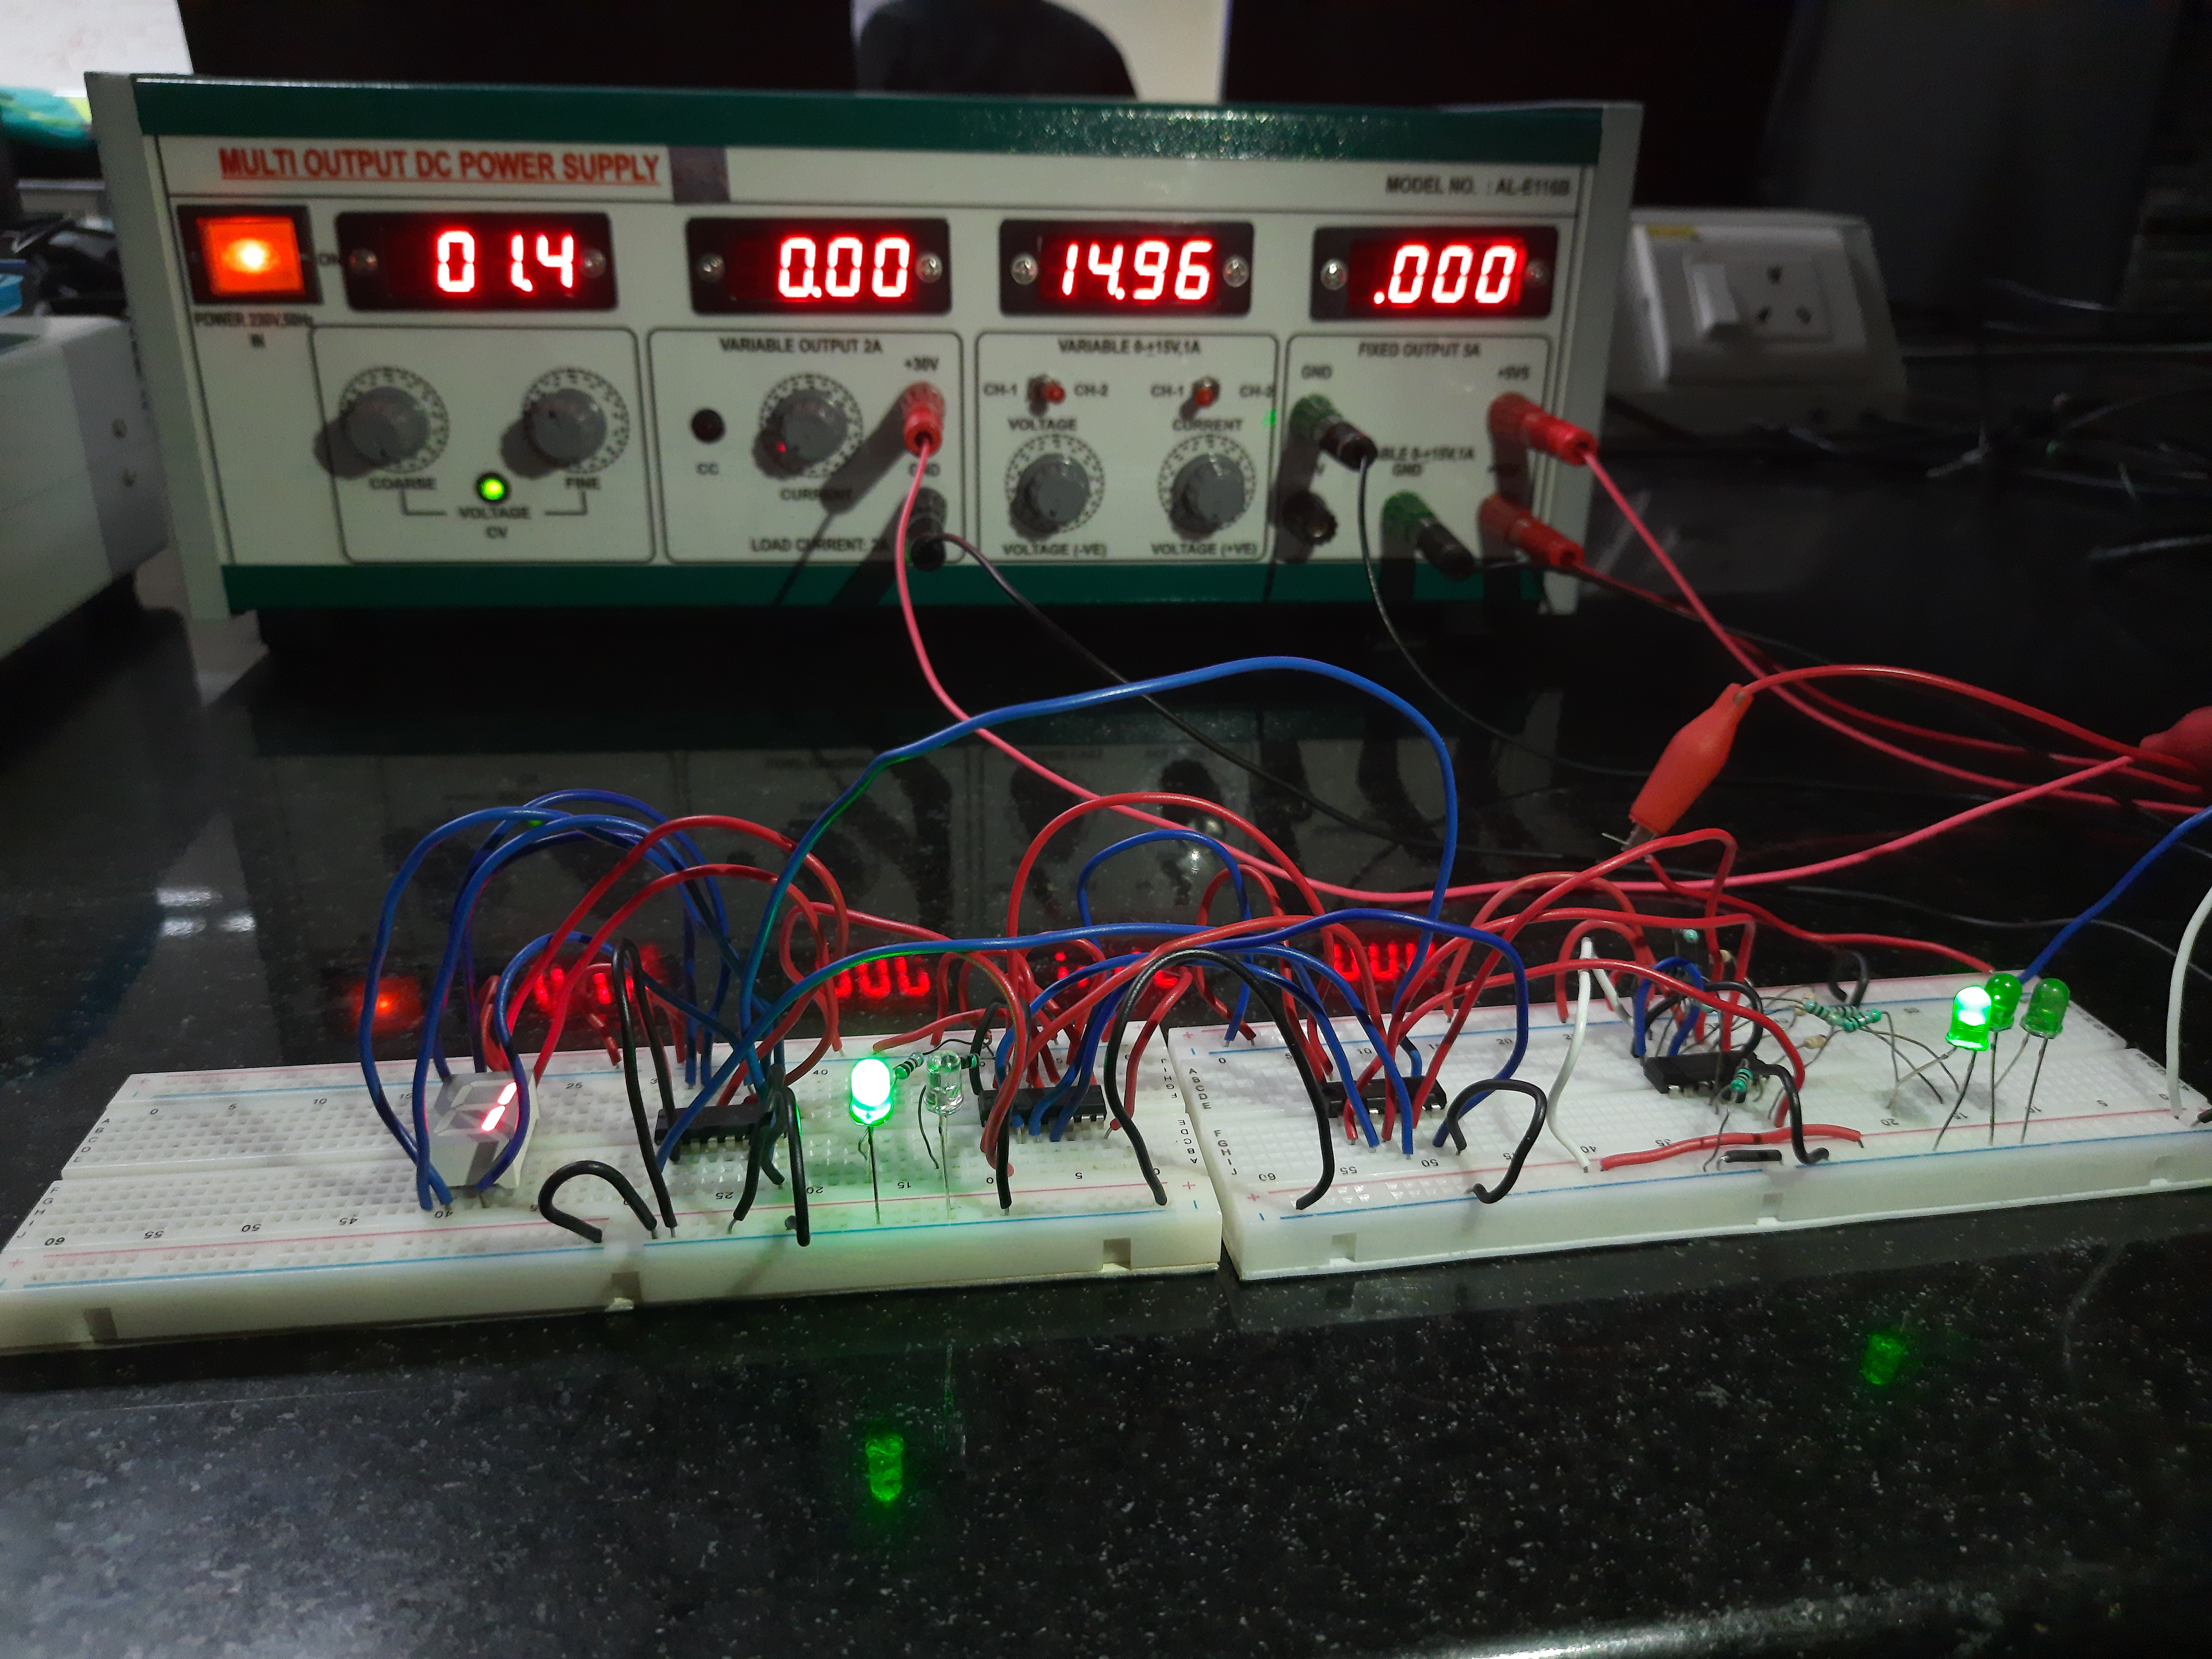
\includegraphics[scale=0.8]{1} 
	\caption{Compton scattering of electrons}
	\label{1}
\end{figure}
For $\theta=0$, Compton wavelength is defined as h/me=.02426 \AA. 

Substituting Planck's equation in (\ref{e1}), we get,
\begin{equation}\label{e2}
	E_\theta=\frac{E_o}{1+\gamma(1-cos\theta)}
\end{equation}

For $\theta=0$, Compton wavelength ($\lambda_c$) is defined as h/me=.02426 \AA. 

For photons with energy greater than 511 keV, the wavelength of the scattered radiation is of the order of $\lambda_c$, otherwise the change is small. The differential Compton scattering cross section area was formulated by Klein and Nishina wgich is given by:
\begin{equation}\label{e3}
	\frac{d\sigma}{d\Omega}=\frac{r_o^2(1+cos^2\theta)}{2(1+\gamma(1-cos\theta))^2}\left( 1+\frac{(\gamma(1-cos\theta))^2}{(1+cos^2\theta)(1+\gamma(1-cos\theta))}\right) 
\end{equation}

where $r_o$=e/4$\pi$$\epsilon_o$$m_e c^2$=2.8179$\times$$10^{-15}$ m is the classical electron radius. Integrating the equation (\ref{e3}), we obtain the total cross section area. From this, we can also calculate Calibration factor C as :
\begin{equation}\label{e4}
	C=\frac{1}{n}\sum_{\theta=0}^{n}\frac{I_\theta}{\frac{d\sigma}{d\Omega}}
\end{equation}

where $I_\theta$ is the relative intensity of the scattered radiation peaks.

\section{Experiment}
The experimental setup is as shown in figure (\ref{setup}). To calibrate we use mixed nuclide source of $\text{Am}^{241}$ and $\text{Cs}^{137}$. After the energy levels are calibrated, The radioactive source of $\text{Cs}^{137}$ produces 661.66 keV $\gamma$ rays which can escape shielded lead cavity to collimate and hit the scatterer (brass and aluminium), where some portion of the rays get scattered by the electrons in the target which are detected in NaI scintillation counter. Set the operating voltage as 0.7 kV in the voltage source to the detector. The signal is processed by MCA and spectrum is viewed in CASSY lab software and analysed. Repeat the process of scattering at various angles by using the lead block to obstruct the direct gamma rays hitting the detector. The scattered radiations collected to study the angular dependence Compton scattering. Fit the function with the Gaussian equal width, for each scattering spectra and parameters, and determine the area under the peak to get relative intensities. The calibration factor can be calculated by equation (\ref{e4}). To free fit the plot for energy versus scattering angle, use the following function:

\begin{equation}\label{ff}
	\frac{661.66}{1+661.66(1-cos\theta)/511}
\end{equation}

To find the rest mass of electron, replace 511 keV by a constant to get the parameter.
\begin{figure}[H]
	\centering
	\includegraphics[height=5cm, width=8cm]{setup} 
	\caption{Experimental setup for Compton scattering in laboratory.}
	\label{setup}
\end{figure}

\section{Observation and Analysis}

% Please add the following required packages to your document preamble:
% \usepackage{graphicx}
\begin{table}[H]
	\centering
	\caption{Observations for Aluminium Scatterer}
	\label{t1}
	\text{$\gamma_{Al}=1.44~~~~~~~C_{avg}=4.41\times10^{32}$}
	\resizebox{\columnwidth}{!}{%
		\begin{tabular}{|r|r|r|r|l|r|r|}
			\hline
			\multicolumn{1}{|l|}{$\theta$(in deg)} &
			\multicolumn{1}{l|}{$cos \theta$} &
			\multicolumn{1}{l|}{E (keV)} &
			\multicolumn{1}{l|}{$E_{\theta}$ (keV)} &
			$\frac{d\sigma}{d\Omega}$ ($m^2$) &
			\multicolumn{1}{l|}{$I_{\theta}$} &
			\multicolumn{1}{l|}{C=$\frac{I_{\theta}}{\frac{d\sigma}{d\Omega}}$} \\ \hline
			0   & 1     & 660.7 & 660.7  & 7.94E-30 & 14386 & 1.81E+33 \\ \hline
			30  & 0.866 & 551.7 & 468.26 & 5.08E-30 & 865   & 1.70E+32 \\ \hline
			45  & 0.707 & 470.2 & 338.38 & 3.31E-30 & 432.5 & 1.31E+32 \\ \hline
			60  & 0.5   & 391   & 234.83 & 2.17E-30 & 468   & 2.16E+32 \\ \hline
			90  & 0     & 280.5 & 120.38 & 1.28E-30 & 269.5 & 2.10E+32 \\ \hline
			120 & -0.5  & 213.1 & 71.15  & 1.14E-30 & 122.5 & 1.08E+32 \\ \hline
		\end{tabular}%
	}
\end{table}

% Please add the following required packages to your document preamble:
% \usepackage{graphicx}
\begin{table}[H]
	\centering
	\caption{Change in Wavelength for Aluminium}
	\label{t2}
	\resizebox{\columnwidth}{!}{%
		\begin{tabular}{|r|r|r|r|r|r|}
			\hline
			\multicolumn{1}{|l|}{$\theta$(in deg)} &
			\multicolumn{1}{l|}{$cos \theta$} &
			\multicolumn{1}{l|}{E (keV)} &
			\multicolumn{1}{l|}{$E_{\theta}$ (keV)} &
			\multicolumn{1}{l|}{$\Delta E$ (keV)} &
			\multicolumn{1}{l|}{$\Delta \lambda$ (\AA)} \\ \hline
			0.00   & 1.00  & 660.70 & 660.70 & 0.00   & 0.00 \\ \hline
			30.00  & 0.87  & 551.70 & 468.26 & 83.44  & 0.05 \\ \hline
			45.00  & 0.71  & 470.20 & 338.38 & 131.82 & 0.13 \\ \hline
			60.00  & 0.50  & 391.00 & 234.83 & 156.17 & 0.27 \\ \hline
			90.00  & 0.00  & 280.50 & 120.39 & 160.11 & 0.76 \\ \hline
			120.00 & -0.50 & 213.10 & 71.15  & 141.95 & 1.52 \\ \hline
		\end{tabular}%
	}
\end{table}

% Please add the following required packages to your document preamble:
% \usepackage{graphicx}
\begin{table}[H]
	\centering
	\caption{Standard Deviation calculation for C for Aluminium. $\sigma=6.14\times10^{32}$}
	\label{er2}
	\resizebox{\columnwidth}{!}{%
		\begin{tabular}{|r|r|r|}
			\hline
			\multicolumn{1}{|l|}{\begin{tabular}[c]{@{}l@{}}Calibration  factor $(C_i)$\end{tabular}} &
			\multicolumn{1}{l|}{$C_{i} - C_{avg}$} &
			\multicolumn{1}{l|}{$(C_{i} - C_{avg})^2$} \\ \hline
			1.81E+33 & 1.37E+33  & 1.88E+66 \\ \hline
			1.70E+32 & -2.71E+32 & 7.33E+64 \\ \hline
			1.31E+32 & -3.10E+32 & 9.63E+64 \\ \hline
			2.16E+32 & -2.25E+32 & 5.07E+64 \\ \hline
			2.10E+32 & -2.31E+32 & 5.34E+64 \\ \hline
			1.08E+32 & -3.33E+32 & 1.11E+65 \\ \hline
		\end{tabular}%
	}
\end{table}

% Please add the following required packages to your document preamble:
% \usepackage{graphicx}
\begin{table}[H]
	\centering
	\caption{Observations for Brass scatterer}
	\text{$\gamma_{Brass}=1.24~~~~~~~C_{avg}=7.01\times10^{32}$}
	\label{t3}
	\resizebox{\columnwidth}{!}{%
		\begin{tabular}{|r|r|r|r|r|r|r|}
			\hline
			\multicolumn{1}{|l|}{$\theta$(in deg)} &
			\multicolumn{1}{l|}{$cos \theta$} &
			\multicolumn{1}{l|}{$E$ (keV)} &
			\multicolumn{1}{l|}{$E_{\theta}$ (keV)} &
			\multicolumn{1}{l|}{$\frac{d\sigma}{d\Omega}$ ($m^2$)} &
			\multicolumn{1}{l|}{$I_{\theta}$} &
			\multicolumn{1}{l|}{$C=\frac{I_{\theta}}{\frac{d\sigma}{d\Omega}}$} \\ \hline
			0   & 1     & 662.9 & 662.90 & 3.41E-30 & 7521  & 2.21E+33 \\ \hline
			30  & 0.866 & 555.7 & 471.66 & 2.25E-30 & 1095  & 4.87E+32 \\ \hline
			45  & 0.707 & 486.3 & 349.97 & 1.33E-30 & 951   & 7.14E+32 \\ \hline
			60  & 0.5   & 413.1 & 248.11 & 1.19E-30 & 841   & 7.06E+32 \\ \hline
			90  & 0     & 296.1 & 127.08 & 7.94E-30 & 524.5 & 6.60E+31 \\ \hline
			120 & -0.5  & 228.1 & 76.16  & 7.94E-30 & 239.5 & 3.02E+31 \\ \hline
		\end{tabular}%
	}
\end{table}

% Please add the following required packages to your document preamble:
% \usepackage{graphicx}
\begin{table}[H]
	\centering
	\caption{Change in Wavelength for Brass}
	\label{t4}
	\resizebox{\columnwidth}{!}{%
		\begin{tabular}{|r|r|r|r|r|r|}
			\hline
			\multicolumn{1}{|l|}{$\theta$(in deg)} &
			\multicolumn{1}{l|}{$cos \theta$} &
			\multicolumn{1}{l|}{$E$ (keV)} &
			\multicolumn{1}{l|}{$E_{\theta}$ (keV)} &
			\multicolumn{1}{l|}{$\Delta E$ (keV)} &
			\multicolumn{1}{l|}{$\Delta \lambda$ (\AA)} \\ \hline
			0   & 1            & 662.9 & 662.90 & 0.00   & 0.00 \\ \hline
			30  & 0.866 & 555.7 & 471.66 & 84.04  & 0.05 \\ \hline
			45  & 0.707 & 486.3 & 349.97 & 136.33 & 0.12 \\ \hline
			60  & 0.5          & 413.1 & 248.11 & 164.99 & 0.24 \\ \hline
			90  & 0            & 296.1 & 127.08 & 169.02 & 0.66 \\ \hline
			120 & -0.5         & 228.1 & 76.16  & 151.94 & 1.28 \\ \hline
		\end{tabular}%
	}
\end{table}

% Please add the following required packages to your document preamble:
% \usepackage{graphicx}
\begin{table}[H]
	\centering
	\caption{Standard Deviation calculation for C for brass. $\sigma=7.25\times10^{32}$}
	\label{er1}
	\resizebox{\columnwidth}{!}{%
		\begin{tabular}{|r|r|r|}
			\hline
			\multicolumn{1}{|l|}{\begin{tabular}[c]{@{}l@{}}Calibration factor $(C_i)$\end{tabular}} &
			\multicolumn{1}{l|}{$C_{i} - C_{avg}$} &
			\multicolumn{1}{l|}{$(C_{i} - C_{avg})^2$} \\ \hline
			2.20508E+33 & 1.50408E+33  & 2.26226E+66 \\ \hline
			4.87013E+32 & -2.13987E+32 & 4.57903E+64 \\ \hline
			7.14054E+32 & 1.30543E+31  & 1.70415E+62 \\ \hline
			7.06089E+32 & 5.0894E+30   & 2.5902E+61  \\ \hline
			6.60486E+31 & -6.34951E+32 & 4.03163E+65 \\ \hline
			3.01595E+31 & -6.70841E+32 & 4.50027E+65 \\ \hline
		\end{tabular}%
	}
\end{table}

The scattering spectra for Aluminium and Brass is as shown in figures (\ref{als}) and (\ref{bs}).

\begin{figure}[H]
	\centering
	\includegraphics[width=\columnwidth]{al spectra} 
	\caption{Compton scattering spectra with aluminium as scatterer.}
	\label{als}
\end{figure}

\begin{figure}[H]
	\centering
	\includegraphics[width=\columnwidth]{br spectra} 
	\caption{Compton scattering spectra with brass as scatterer.}
	\label{bs}
\end{figure}

From the free fit of plot of Energy versus scattering angle shown in figure(\ref{aem}) and figure (\ref{bem}), we obtain the electron mass as 458.86 keV for the case of aluminium as scatterer whereas from brass we get 531.92 keV giving the average electron mass as 495.39 keV. The percentage error is rest mass of electron is 3.05\% with the reference value as 511 keV. 

\begin{figure}[H]
	\centering
	\includegraphics[width=\columnwidth]{al fit} 
	\caption{Free Fit for Aluminium to determine electron mass from equation (\ref{ff}). A (electron mass)=458.86 keV}
	\label{aem}
\end{figure}

\begin{figure}[H]
	\centering
	\includegraphics[width=\columnwidth]{br fit} 
	\caption{Free Fit for Brass to determine electron mass from equation (\ref{ff}). A (electron mass)=531.92 keV}
	\label{bem}
\end{figure}

\section{Conclusion}
We studied the angular dependence of energy of the scattered particles by the Compton effect using aluminium and brass as scatterers with Cs-137 as gamma ray source. The differential cross section area was calculated from Klein-Nishina's formula. The mean rest mass of electron was found out from the scattering spectra to be $495.39\pm3.05\%$ keV from the free fit with the energy of scattered rays. $\gamma_{Al}$ and $\gamma_{Brass}$ was found as 1.44 and 1.24, respectively. We also estimated the calibration factor as $4.41\times10^{32}$ and $7.01\times10^{32}$ former and latter case, respectively. The standard deviation for each case was $6.14\times10^{32}$ and $ 7.25\times10^{32}$, respectively. 

It should be noted that the direct radiations from the source should be obstructed by lead block as they may interfere with the spectra contributing to the errors in the experiment. Background radiation and unnecessary mechanical disturbances to the setup may add noise to the spectra. Also collimating the gamma ray at particular angle is necessary in order to reduce errors. This experiment was success in determining the rest mass of electron within 3.05\% of the literature value. 

\section{References}
\begin{enumerate}
\item{{Lab Handout}}
\item{\url{http://hyperphysics.phy-astr.gsu.edu/hbase/quantum/comptint.html}}
\end{enumerate}

\end{document}